\section{Introduction}
\label{sec:intro}

The widespread adoption of Internet of Things (IoT) technologies, industrial monitoring
systems, and real-time financial applications has generated an unprecedented volume of
temporal data, creating critical challenges for storage and analysis infrastructures.
As projected by~\cite{thierer2015iot}, the number of connected IoT devices has been growing
exponentially and is expected to continue increasing in the coming years, as illustrated in
Figure~\ref{fig:iot_projection}.

\begin{figure}[ht]
  \centering
  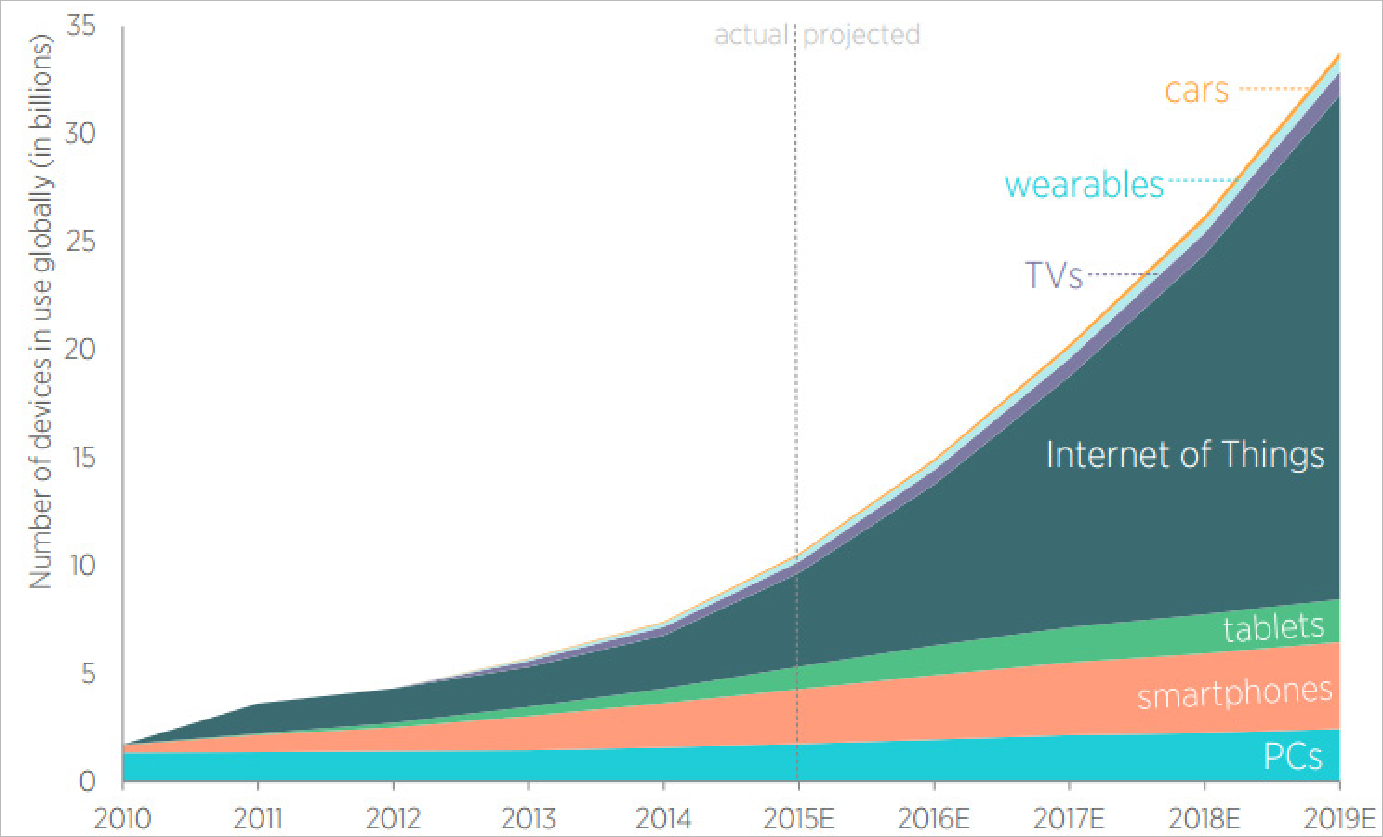
\includegraphics[width=\columnwidth]{figures/en_us/projecao-iot}
  \caption{IoT: devices in use globally. Source:~\cite{thierer2015iot}.}
  \label{fig:iot_projection}
\end{figure}

This growth trajectory was subsequently reaffirmed by~\cite{zikria2021nextgen}, who reports that Cisco forecasts 500 billion devices connected to the IoT by 2030, while Telefonica estimates that 90\% of vehicles will be connected and each person will have an average of 15 connected devices by the same horizon. The proliferation of next-generation applications, spanning smart healthcare, smart cities, smart agriculture, and industrial IoT, confirms that the projections made in 2015 not only materialized but continue to expand.

As noted by~\cite{palma2016}, numerous sectors have come to depend on the ability to process
continuous data streams. Among them: the financial sector, which relies on this capability to
analyze stock fluctuations and transaction volumes; transportation services, which employ it to
monitor trips and seasonal migrations; medicine, which uses it to track the spread of diseases;
and meteorological analysis, which leverages historical data for more accurate forecasts.

These data streams are sequences of events or measurements that are naturally ordered and indexed
by time, often with millisecond precision. As observed by~\cite{Dunning2014}, what used to take
ten minutes to collect for some very active systems is now generated every second. This explosion
of time-indexed sequential data exposed the fundamental limitations of traditional relational
databases when confronted with temporal access patterns, high-velocity ingestion, and efficient
long-term historical storage.

In this scenario, Time Series Databases (TSDBs) emerged as specialized solutions, architected
from the ground up to meet the unique demands of temporal data~\citep{InfluxDataTimeSeries}.
As argued by~\cite{naqvi2017influxdb}, traditional relational databases suffer from indexing
inefficiencies and memory limitations when dealing with large volumes of temporal data, whereas
TSDBs maintain high performance because they were built to treat time as their primary concern.
Beyond raw throughput, TSDBs offer specialized compression mechanisms, time-interval data
co-location, and automatic retention policies that reduce operational costs, features that
are indispensable for IoT applications where continuous sensor measurements demand scalability
and economical resource usage~\citep{Dunning2014}.

The TSDB landscape has expanded in recent years, with systems adopting distinct
architectural approaches to the same problem. \textit{Apache IoTDB}~\cite{wang2023iotdb},
developed at Tsinghua University, is purpose-built for industrial IoT, using a custom columnar
file format (TsFile) and a binary RPC protocol that enables extremely high ingestion rates.
\textit{InfluxDB}, evaluated in four of the five performance studies reviewed in this
work~\citep{naqvi2017influxdb,shah2022performance,lima2024avaliando,wang2023iotdb}, uses a
Time-Structured Merge Tree (TSM) engine exposed via an HTTP line-protocol API. \textit{TimescaleDB}
extends PostgreSQL with time-series capabilities~\citep{Ramakrishnan2003}, offering SQL compatibility
and the full relational ecosystem as trade-offs for lower raw write throughput. Each approach has
distinct strengths and weaknesses that are not apparent from descriptions alone and require
controlled measurement under realistic IoT workloads.

The field of TSDB benchmarking, however, suffers from a critical methodological gap: the lack of
reproducibility. A survey of recent comparative studies reveals that the majority of published
benchmarks do not provide sufficient scripts, configurations, or exact software versions to
allow independent replication~\citep{pereira2023mulletbench,shah2022performance,naqvi2017influxdb}.
Without reproducible methodology, findings cannot be independently validated, results are
difficult to compare across studies, and experiments cannot be adapted to new hardware or
software versions. This work directly addresses that gap by making the complete benchmark
infrastructure (all orchestration scripts, container definitions, build environment, and
parameterized benchmark clients) publicly available alongside the results.

This paper presents a controlled, reproducible comparison of Apache IoTDB, InfluxDB~2.7,
and TimescaleDB across nine workload patterns representative of IoT deployments and three
data-volume scales. The databases were selected based on their prominence in recent comparative
literature: InfluxDB as the established reference standard, Apache IoTDB as the emerging leader
in the two most recent studies~\citep{pereira2023mulletbench,wang2023iotdb}, and TimescaleDB as
the SQL-based alternative that provides broad ecosystem compatibility. The benchmark methodology
is designed to isolate architectural properties from measurement artefacts, including an
explicit comparison between original shared-resource runs and isolated, properly tuned reruns
to validate which findings reflect genuine database behavior.

The specific objectives of this work are:
\begin{itemize}
  \item Measure write and read performance of three TSDBs across workloads representative of
    real IoT deployments;
  \item Analyze how performance characteristics scale with data volume across three scales
    spanning a hundredfold range in data size;
  \item Identify the architectural mechanisms that explain the observed performance differences;
  \item Quantify the impact of benchmark methodology choices on reported results; and
  \item Provide a reproducible benchmark infrastructure that enables future researchers to
    independently validate and extend these results.
\end{itemize}

The remainder of this paper is organized as follows.
Section~\ref{sec:theoretical} presents the theoretical foundations covering databases,
time series databases, and benchmarking concepts.
Section~\ref{sec:related} reviews related comparative studies and identifies the gaps that
motivate this work.
Section~\ref{sec:methodology} describes the benchmark methodology, workload design, and
reproducible infrastructure.
Section~\ref{sec:experiments} presents and analyzes the experimental results.
Section~\ref{sec:conclusion} concludes the paper with a final comparison and directions
for future work.
